% Time series analysis appendix. 

\par \indent Cohen's paper \cite{CohenSelfControl} discusses analyzing the 
data with time series using FILM (FMRIBs Improved Linear Model). While we are 
not familiar with the FILM method, we did try modeling individual voxels in 
the framework of an autoregressive integrated moving average (ARIMA) process. 
We focused only on a single voxel from the first subject, but the method 
could easily be extended to additional or aggregate voxels. Let $\{Y_t\}$ be 
a single volume's value at time $t$ and assume that the $d$th difference 
$W_t = \nabla^d Y_t$ is weakly stationary, defined to be when $W_t$ has a 
constant mean function and autocovariance dependent only on lag $k$ and not 
time $t$. Then we can try to model $W_t$ as a linear combination of $p$ 
autoregressive terms (or the number of most recent values to include) and $q$ 
moving average terms (the number of lags to include for the white noise error 
terms): 
$$W_t = \phi_1 W_{t-1} + \phi_2 W_{t-2} + ... + \phi_p W_{t-p} + e_t - 
\theta_1 e_{t-1} - \theta_2 e_{t-2} - ... - \theta_q e_{t-q}.$$

\par White noise is defined as a sequence of independent, identically 
distributed random variables. In order to fit an ARIMA process, the three 
orders $p$, $d$, and $q$ must be first be specified, and the the associated 
coefficients estimated. We used a combination of visual inspection and 
quantitative methods to specify the ARIMA orders, and then used the maximum 
likelihood method to estimate parameters. 

\par Having specified the order for $d$, we turned to the problem of 
specifying $p$ and $q$. We used a combination of visually inspecting the 
autocorrelation and partial autocorrelation plots of the first difference, 
and looking at the Akaike information criteria (AIC) and Bayesian information 
criteria (BIC) computed from a grid of possible models. The latter method 
suggested specifying $p=1$ and $q=1$ (based on either the AIC or the BIC), 
which was also supported by the visual inspections. 

\par We estimated the parameters for an ARIMA(1,1,1) model using the exact 
maximum likelihood estimator via Kalman filter. The residuals appear to be 
normally distributed, and its autocorrelation and partial autocorrelation 
plots also do not raise any red flags. Furthermore, when visually comparing 
the fitted time series to the true observed data, the ARIMA process seems to 
approximate the observed data much better than any of the linear regression 
models. However, since specifying the correct ARIMA process orders and 
estimating the associated parameters must be done separately by hand for 
each individual voxel of interest, we decided to eliminate this direction 
of analysis from our main pipeline. 

\par Had we decided to continue pursuing time series analysis, we may have 
tried to forecast future observations based on previous ones. As an example, 
we modeled an ARIMA(1,1,1) process based on the first half of the 
observations for a single voxel. This process was then used to forecast the 
second half of the observations. A comparison between the true observations 
and the forecasted predictions is shown in [Figure \ref{fig:ts-preds}]. 
While the forecasted observations look reasonable for approximating the true 
values, more quantitative and robust metrics for assessing performance need 
to be implemented. 

\begin{figure}[ht]
\centering
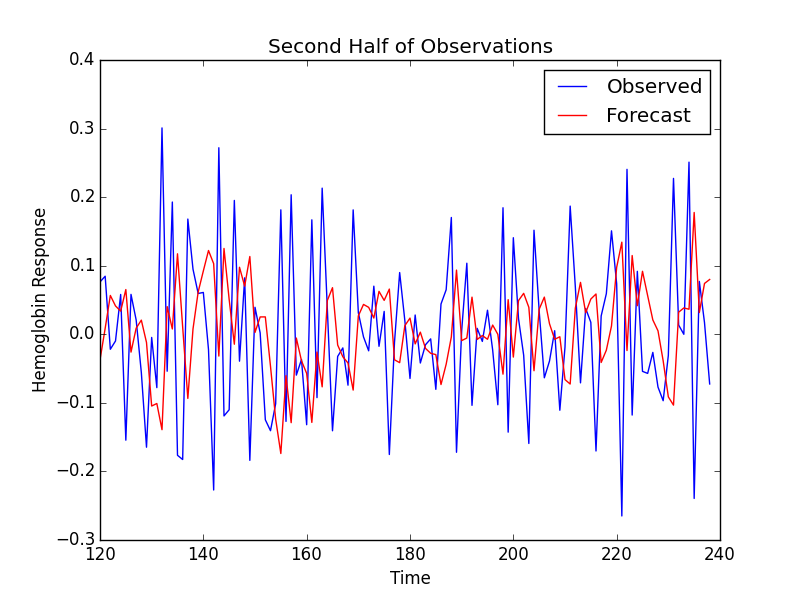
\includegraphics[scale=0.5]{../images/ts-preds.png}
\caption{Forecasting the second half of observations based on the first 
half.}
\label{fig:ts-preds}
\end{figure}

\par One such procedure for assessing performance would be to design a 
permutation test. A null voxel time course could be simulated from by 
performing a Fourier transform on the observed time course, permuting the 
phases, and then transforming back to the original space. That way, the 
simulated time course has the same autocovariance as the observed time 
course, but random signal (as under the null case). We can then fit the 
same ARIMA model to the permuted process and examine how much, if at all, 
the ARIMA process fitted to the observed data makes improvements over the 
null case. Generating confidence intervals for the parameter estimates and 
forecasting future observations may also be of interest. Other considerations 
for modeling voxels as time series include exploring efficient and 
reasonable techniques for comparing multiple voxels both within and across 
subjects. 

\par Other approaches for modeling time series could also be considered, 
such as spectral density or modeling the conditional variance instead of the 
conditional mean with an ARCH (autoregressive conditional 
heteroskedasticity) model. 

\bibliography{project}

\end{document}
